\newglossaryentry{Charles D. Moore}
{
  name={Charles D. Moore},
  description={Charles D. Moore, is the inventor of the forth programming language.}
}

\chapter{Results}
\label{chap:Results}

In this chapter, I will introduce the chosen forth software. Afterwards, I will manually or semi automatically produce the graphics according to the selected Visualization methods.

\section{The software under investigation: Brainless}

Brainless\footnote{Brainless verion 0.1.2 is used, the source code can be optained on \url{http://sourceforge.net/projects/forth-brainless/}} is chess-playing program written in ANS Forth. The source code consists of several files with an overall size\footnote{The command to calculate the size was \emph{find . -name '*.fs' -maxdepth 1 | xargs wc -l}} of about 139497 bytes and 4108 lines of code\footnote{The command used to count the lines of code, was \emph{find . -name '*.fs' -maxdepth 1 | xargs wc -l}}.
This measure is somehow controversial, but since the files contain only a short header and are formatted in the usual manner, it seems appropriate for comparison.

The other software, I took into consideration, was brew\footnote{brew version 0.2.0 was used. The source code can be obtained on \url{http://www.robertepprecht.ch/brew/index.html}}. Brew is a 'playground for evolutionary programming', as the author calls it. Due to its size of 1062857 bytes and 36801 lines of code, this project seem to large to analyze manually in a reasonable time.

\section{The application of the previously presented methods}

\subsection*{Hierarchical edge bundles}

The source code of brainless is organizes in a flat structure, there is only one directory, which contains all the source files.

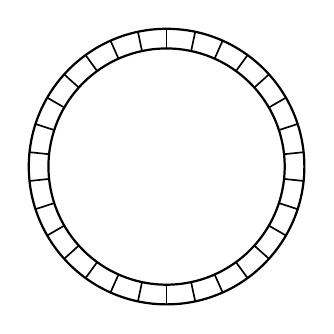
\begin{tikzpicture}[>=latex,font=\sffamily,semithick,scale=1.75]
    \draw [thick] (0,0) circle (1);
    \foreach \angle in {90,78,...,-78}
        \draw (\angle:1) -- (\angle-180:1);
    \node [circle,thick,fill=white,draw=black,align=center,minimum size=3cm] at (0,0) {};
    (Head.west);
\end{tikzpicture}


There is only one word list created by brainless, so the hierarchy utilizing the search order would be as follows.


\hl{In context of forth, word execution can be mapped to non hierarchic relations and directory/file tree and the definition could be the hierarchic relations. Like in object oriented systems, the proper organization of directories, files and word definitions has to be considered to make such a visualization helpful.
Another possible mapping could depend on word list as words hierarchic and word execution as non hierarchic relation.}

\subsection*{Information murals and massive sequence view}
The information mural was initially proposed by \cite{Jerding:1998:IMT:614271.614408}. A modified version, mass sequence view proposed by \cite{Cornelissen2009}, which turns the horizontal scrolling into vertical scrolling and also contains the hierarchic aspect could be more suitable. As with the hierarchical edge bundles, the usefulness of the hierarchical component depends highly on the organization of the software at hand.
\\
In the following chapter I will analyze the massive sequence view using a real forth software as an example.

\subsection*{High-Level polymetric views}
Polymetric views\cite{Ducasse:2004:HPV:977397.977739} are a very interesting and approach to grasp the behavior of very large systems. In polymetric views, system attributes or measures are mapped to attributes of a graph. The attributes proposed by\cite{Ducasse:2004:HPV:977397.977739}, are position, height, width, color and the relations(and the thickness) between rectangles, representing aspects of the software to analyze. In terms of forth, the mapping to words seems most obvious. This would result in some kind of a word cloud with more information attached. This could be most valuable, when used with the appropriate metrics, to analyze and optimize performance. Another advantage is, that there is no complete, but  only condensed data required.
\\
In the following chapter I will analyze forms of polymetric views of real software as an example.

\subsection*{Fisheye views}
Fisheye views were first proposed by \cite{Furnas:1986:GFV:22627.22342} and formulated by \cite{Storey:1995:GLA:647547.728600} and \cite{Sarkar:1994:GFV:198366.198384}. The essence of fisheye views is a principle found in nature. It's basically described as a function, expressing the degree of interest of an subject, depending on an a priori importance and the distance from the current point of view. With growing distance lowers the degree of interest.
\\
This method is related to polymetric views, as mentioned above.

\subsection*{Execution pattern view}
The execution pattern view proposed by \cite{Pauw98executionpatterns} to visualize large traces in a scalable manner and helps to identify execution patterns, represent an interesting evolution of simple sequence diagrams and interaction diagrams.
\\
Since it is somehow related to the massive sequence view, I will not pursue this approach in detail.

\subsection*{Method invocation view and taxonomy view}
The tool \gls{GraphTrace}\cite{Kleyn:1988:GOS:62084.62101} is meant to analyze object oriented programs. I provides a method invocation view and a taxonomy view. Although the method invocation approach of GraphTrace seems not practical for forth programs, the authors mentioned two very interesting ideas.
\begin{itemize}
\item Displaying variable access:\\
	The idea of showing words which access variables and the other way round, showing which words access a specific variable is very interesting. Thus it would be easier to track the global state of a program.
\item Concurrent views:\\
	The authors of \cite{Kleyn:1988:GOS:62084.62101} present a quiet interesting analogy. They compare the execution of a program with a tennis and football and refer to the multiple perspectives necessary to understand all aspects of a match and the whole outcome.
\end{itemize}

In the following chapter I will create a variable access graph inspired by the tree like visualization of GraphTrace.

\subsection*{Frequency spectrum analysis}

The frequency spectrum analysis as proposed by \cite{Ball:1999:CDA:318774.318944} provides an interesting approach. It is similar to parametric views as mentioned before, but the visualization is not graphical but textual. The word execution frequency could provide valuable information about the actual performed work and incorporated with execution time, it could help in understanding programs and support performance analysis. In \cite{Ball:1999:CDA:318774.318944}, Ball shows the application of frequency spectrum analysis at the example of an obfuscated c program. Although this is not the main focus of this thesis, his approach should also apply to concatenative languages.

In the following chapter I will briefly analyze this approach at an example of a large forth program.

\section{gfvis - A trace visualization enhancement for Gforth}

\hl{TODO put this under the matching viz methods!!}
A very important question in this concern is, how can developers be assisted to write readable code. Experienced developers may do that intuitively, but how can novice developers be encouraged and supported to write readable code. Concatenative languages are flexible enough to produce code very similar to natural languages, but how can this attribute be supported?\\
One answer is to provide hints based on static analysis.\\
It is not possible to make every word completely readable and the perceived readability also depends on the experience of the developer. At some point  it always comes down to longer combinations of "nip tuck over rot", this is hardly avoidable at the lowest level. Thus, proper documentation of words is essential. Its pretty The obvious, that stack effect comment\footnote{See \url{https://www.complang.tuwien.ac.at/forth/gforth/Docs-html/Stack\_002dEffect-Comments-Tutorial.html\#Stack\_002dEffect-Comments-Tutorial}} in forth, are a must have, but also the behavior of the word should be explained if complex or not very natural to read words\footnote{Most notable \\G in gforth. See \url{https://www.complang.tuwien.ac.at/forth/gforth/Docs-html/Comments.html\#Comments}}. Another advantage of word definition comments is the possibility of automated documentation generation.\\
Very long word definitions tend increase the amount of brain capacity required to understand its behavior. The way to account this problem is to break down the overall task into manageable pieces. It is called factoring\footnote{See \url{https://www.complang.tuwien.ac.at/forth/gforth/Docs-html/Factoring-Tutorial.html\#Factoring-Tutorial}} in context of concatenative languages. An approach could be to place a hint on word definitions which exceed a certain amount of lines or words or different words and suggest further factoring.\\
Another tool to make code read more natural, is aliasing\footnote{See \url{https://www.complang.tuwien.ac.at/forth/gforth/Docs-html/Aliases.html}}. By defining aliases for a certain word, its functionality can be used in different contexts and still read very natural.
Expressive naming, although obvious, it should be mentioned that assigning expressive and fitting names for words is essential. This applies to any language[does it? cite...].\\
To understand code, the systematic approach turned out to be most efficient\cite{Robillard:2004:EDI:1042203.1042417}. To ease afford of finding the definition of words used at a certain point, a hyperlink like referencing mechanism can be used[cite the visualization paper with the hyperlink feature].\\
As stated by \gls{Charles D. Moore} in \cite{Biancuzzi:2009:MPC:1592983}: "... The challenge there is 1) deciding
which words are useful, and 2) remembering them all.", when programs get larger, the amount of words can grow big. Thus it is suggested to have some sort of a dictionary to search the whole vocabulary by name, stack effect comment, word definition documentation and provide a reverence to where they are used. Auto completion can also help a lot in finding words previously defined.

\begin{itemize}

\item other data structures and variables should be displayed
	\begin{itemize}
	\item memory maybe like \cite{ReissProgrammingEnvironments1995} or \cite{Aftandilian:2010:HIH:1879211.1879222} but since there is no underlying object orientation and no standardized oo system this would be hard do accomplish
	\item fisheye or word cloud like display(tree or sugiyama as of \cite{Storey:1997:IVT:857188.857642})
	\end{itemize}


\item interactive program manipulation: state of the system before a word, after a word and by clicking on the word jumping to its definition or inserting it and there also providing those features

\item stepping debugger mode: simply stepping through the whole code word by word

\item goal-oriented strategy: the definition of an execution scenario such that only the parts of interest of the software system are analyzed (Koenemann and Robertson, 1991; Zaidman,
2006).

\item code analysis and visualization facilities see chapter 2 TODO
\end{itemize}

\subsection{software maintenance}

\begin{itemize}
\item types of maintenance
\item find bugs and fix them
\item find the right place to implement a new feature.
\item find the right place to modify a feature.
\end{itemize}

\subsection{program comprehension}

\begin{itemize}
\item structured approach
\item thorough reading is the most efficient[cite]
\item about the mental model building
\item keeping the mental model up to date
\item keeping artifacts up to date
\end{itemize}


